%%%%%%%%%%%%%%%%%%%%%%%%%%%%%%% beamer %%%%%%%%%%%%%%%%%%%%%%%%%%%%%%%%%%%%%%%%%%%%%%%%%
% To run - pdflatex filename.tex
%      acroread filename.pdf
%%%%%%%%%%%%%%%%%%%%%%%%%%%%%%%%%%%%%%%%%%%%%%%%%%%%%%%%%%%%%%%%%%%%%%%%%%%%%%%%%%%%%%%%

\documentclass[compress,oilve]{beamer}
\mode<presentation>

\usetheme[]{CambridgeUS}
% other themes: AnnArbor, Antibes, Bergen, Berkeley, Berlin, Boadilla, boxes, CambridgeUS, Copenhagen, Darmstadt, default, Dresden, Frankfurt, Goettingen,
% Hannover, Ilmenau, JuanLesPins, Luebeck, Madrid, Maloe, Marburg, Montpellier, PaloAlto, Pittsburg, Rochester, Singapore, Szeged, classic

\usecolortheme{beaver}
% color themes: albatross, beaver, beetle, crane, default, dolphin,  fly, lily, orchid, rose, seagull, seahorse, sidebartab, whale, wolverine

\usefonttheme{professionalfonts}
% font themes: default, professionalfonts, serif, structurebold, structureitalicserif, structuresmallcapsserif


\hypersetup{pdfpagemode=FullScreen} % makes your presentation go automatically to full screen

% define your own colors:
\definecolor{Red}{rgb}{1,0,0}
\definecolor{Blue}{rgb}{0,0,1}
\definecolor{Green}{rgb}{0,1,0}
\definecolor{magenta}{rgb}{1,0,.6}
\definecolor{lightblue}{rgb}{0,.5,1}
\definecolor{lightpurple}{rgb}{0.8, 0.6, 0.9}
\definecolor{gold}{rgb}{.6,.5,0}
\definecolor{orange}{rgb}{1,0.4,0}
\definecolor{hotpink}{rgb}{1,0,0.5}
\definecolor{newcolor2}{rgb}{.5,.3,.5}
\definecolor{newcolor}{rgb}{0,.3,1}
\definecolor{newcolor3}{rgb}{1,0,.35}
\definecolor{darkgreen1}{rgb}{0, .35, 0}
\definecolor{darkgreen}{rgb}{0, .6, 0}
\definecolor{darkred}{rgb}{.75,0,0}
\definecolor{skyblue}{HTML}{75bbfd}

\definecolor{olive}{cmyk}{0.64,0,0.95,0.4}
\definecolor{purpleish}{cmyk}{0.75,0.75,0,0}

% can also choose different themes for the "inside" and "outside"

% \usepackage{beamerinnertheme_______}
% inner themes include circles, default, inmargin, rectangles, rounded

% \usepackage{beamerouterthemesmoothbars}
% outer themes include default, infolines, miniframes, shadow, sidebar, smoothbars, smoothtree, split, tree


\useoutertheme[subsection=true, height=40pt]{smoothbars}

% to have the same footer on all slides
%\setbeamertemplate{footline}[text line]{STUFF HERE!}
\setbeamertemplate{footline}[text line]{} % makes the footer EMPTY
% include packages
%

%show the page numbers in footnote
%\addtobeamertemplate{navigation symbols}{}{%
%	\usebeamerfont{footline}%
%	\usebeamercolor[fg]{footline}%
%	\hspace{1em}%
%	\insertframenumber/\inserttotalframenumber
%}

\setbeamercolor{footline}{fg=purpleish}
\setbeamerfont{footline}{series=\bfseries}

%add color to curent subsection
\setbeamertemplate{section in head/foot}{\hfill\tikz\node[rectangle, fill=darkred, rounded corners=1pt,inner sep=1pt,] {\textcolor{white}{\insertsectionhead}};}
\setbeamertemplate{section in head/foot shaded}{\textcolor{darkred}{\hfill\insertsectionhead}}

% Remove bullet of subsections
\setbeamertemplate{headline}
{%
	\begin{beamercolorbox}{section in head/foot}
		\insertsectionnavigationhorizontal{\textwidth}{}{}
	\end{beamercolorbox}%
}


% modify headlline, specially headline size
\setbeamertemplate{headline}{%
	\leavevmode%
	\hbox{%
		\begin{beamercolorbox}[wd=\paperwidth,ht=3.5ex,dp=1.125ex]{palette quaternary}%
			\insertsectionnavigationhorizontal{\paperwidth}{}{\hskip0pt plus1filll}
		\end{beamercolorbox}%
	}
}

\setbeamertemplate{footline}{%
	\leavevmode%
	\hbox{\begin{beamercolorbox}[wd=.5\paperwidth,ht=2.5ex,dp=1.125ex,leftskip=.3cm plus1fill,rightskip=.3cm]{author in head/foot}%
			\usebeamerfont{author in head/foot}\insertshortauthor ~ \insertshortinstitute
		\end{beamercolorbox}%
		\begin{beamercolorbox}[wd=.5\paperwidth,ht=2.5ex,dp=1.125ex,leftskip=.3cm,rightskip=.3cm plus1fil]{title in head/foot}%
			\usebeamerfont{title in head/foot}\insertshorttitle\hfill\insertframenumber\,/\,\inserttotalframenumber
	\end{beamercolorbox}}%
	\vskip0pt%
}


%\setbeamertemplate{navigation symbols}{}

\title{Lecture 2: Introduction to ML and Classical Models}
\author{ML Instruction Team, Fall 2022}
\institute[]{CE Department \newline  Sharif University of Technology \newline \newline}
\date[\today]{}
%\titlegraphic{\includegraphics[scale=.35]{example-image}}



%Write \usepackage{etex} just after the \documentclass line (it should be the first loaded package).
\usepackage{etex}
\usepackage{subcaption}
\usepackage{multicol}
\usepackage{physics, amsmath}
\usepackage{epsfig}
\usepackage{graphicx}
\usepackage{amsfonts}
\usepackage{amssymb}
\usepackage[all,knot]{xy}
\xyoption{arc}
\usepackage{url}
\usepackage{multimedia}
\usepackage{hyperref}
\hypersetup{colorlinks,linkcolor=blue,citecolor=redorange,urlcolor=darkred}
\usepackage{multirow}
\usepackage[font={scriptsize}]{caption}
\usepackage{pgf}
\usepackage{fontspec}
\usepackage{subcaption}
\usepackage[export]{adjustbox}
\usepackage{caption}
%\setsansfont[Scale=MatchLowercase, BoldFont = * Bold, ItalicFont = * Italic]{Caladea}
\graphicspath{ {./Pictures/} }
%\usepackage{enumitem,xcolor}
%\newcommand{\labelitemi}{$\blacksquare$}
%\newcommand{\labelitemii}{$\diamond$}
%\newcommand{\labelitemiii}{$\square$}
%\newcommand{\labelitemiv}{$\ast$}
%\setbeamercolor*{item}{fg=red}
\usepackage{bm}

\usefonttheme{professionalfonts} 
\setbeamertemplate{itemize item}{\color{skyblue}$\blacksquare$}
\setbeamertemplate{itemize subitem}{\color{hotpink}$\blacktriangleright$}
\setbeamertemplate{itemize subsubitem}{\color{orange}$\bullet$}


\usepackage{anyfontsize}
\usepackage{t1enc}
\usepackage{tikz}
\usetikzlibrary{calc,trees,positioning,arrows,chains,shapes.geometric,decorations.pathreplacing,decorations.pathmorphing,shapes,matrix,shapes.symbols}



\newtheorem{proposition}[theorem]{Proposition}
\newtheorem{remark}[theorem]{Remark}
\newtheorem{assumption}[theorem]{Assumption}

\usepackage{fontspec,unicode-math}
\setmainfont[Scale=0.9]{Consolas}
\setmonofont[Scale=0.9]{Monaco}
\setsansfont[Scale=1]{Times New Roman}
\newcommand{\vect}[1]{\boldsymbol{#1}}


%\usepackage{smartdiagram}
%\usesmartdiagramlibrary{additions}
%%%%%%%%%%%%%%%%%%%%%%%%%%%%%%%%%%%%%%%%%%%%%%%%%%%%%%%%%%%%%%%%%%%%%%%%%%%%%%%%%%%%%%%%%%%%
%%%%%%%%%%%%%%%%%%%%%%%%%%%%%% Title Page Info %%%%%%%%%%%%%%%%%%%%%%%%%%%%%%%%%%%%%%%%%%%
%%%%%%%%%%%%%%%%%%%%%%%%%%%%%%%%%%%%%%%%%%%%%%%%%%%%%%%%%%%%%%%%%%%%%%%%%%%%%%%%%%%%%%%%%%


%%%%%%%%%%%%%%%%%%%%%%%%%%%%%%%%%%%%%%%%%%%%%%%%%%%%%%%%%%%%%%%%%%%%%%%%%%%%%%%%%%%%%%%%%%
%%%%%%%%%%%%%%%%%%%%%%%%%%%%%% Begin Your Document %%%%%%%%%%%%%%%%%%%%%%%%%%%%%%%%%%%%%%%
%%%%%%%%%%%%%%%%%%%%%%%%%%%%%%%%%%%%%%%%%%%%%%%%%%%%%%%%%%%%%%%%%%%%%%%%%%%%%%%%%%%%%%%%%%
\begin{document}
	
%%%%%%%%%%%%%%%%%%%%%%%%%%%%%%%%%%%%%%%%%%%%%%%%%%%%%%%%%%%%%%%%%%%%%%%%%%%%%%%%%%%%%%%%%%
	\fontsize{9}{9}
\begin{frame}[noframenumbering, plain]
	\titlepage
\end{frame}

%%%%%%%%%%%%%%%%%%%%%%%%%%%%%%%%%%%%%%%%%%%%%%%%%%%%%%%%%%%%%%%%%%%%%%%%%%%%%%%%%%%%%%%%%%
\section{Introduction}
%%%%%%%%%%%%%%%%%%%%%%%%%%%%%%%%%%%%%%%%%%%%%%%%%%%%%%%%%%%%%%%%%%%%%%%%######
\frame{\frametitle{Machine Learning: An Overview}
\begin{center}
What is Machine Learning?
\end{center}
}

%%%%%%%%%%%%%%%%%%%%%%%%%%%%%%%%%%%%%%%%%%%%%%%%%%%%%%%%
\begin{frame}{Machine Learning: An Overview}
\begin{itemize}
\item Let's review some inspirational quotions ... \\
\begin{itemize}
	\item \textit{“Machine learning is the hot new thing”} \\ \begin{center}
— John L. Hennessy, President of Stanford (2000–2016) \end{center}
	\item\textit{ “A breakthrough in machine learning would be worth ten Microsofts” }\\ \begin{center}
— Bill Gates, Microsoft Co-Founder  \end{center}
	\item \textit{“Computers are able to see, hear and learn.  Welcome to the future.” }\\ \begin{center}
— Dave Waters, Professor at University of Oxford \end{center}
	\item \textit{“If software ate the world, models will run it”}
\\ \begin{center}
— Steven A. Cohen and Matthew W. Granade, The Wallstreet Journal, 2018\end{center}
	\item ...
\end{itemize}	
\end{itemize}
\end{frame}

%\begin{frame}{Machine Learning: An Overview}
%\begin{itemize}
%\item[$\blacksquare$] Among these quotions that we have discussed, one seems more interesting and important:\\
%\begin{center} \textit{"Machine learning is the field of study that gives computers the ability to
%learn without being explicitly programmed”} \\ 
%— Arthur L. Samuel, AI pioneer, 1959 \end{center}
%\item[$\blacksquare$] But why does it seem important? why should computers be able to learn? waht do they really learn? \\
%\item[$\blacksquare$] We shall answer these questions through this lecture
%\end{itemize}
%\end{frame}


\begin{frame}{Machine Learning: An Overview}
\begin{itemize}
\item The main motivation which we develop (computer) programs is to automate various
kinds of (often tedious) processes.
\item So far, we have learned to program the computers. the analogy that we are using, is something similar to this:\\

\begin{center}
\begin{figure}
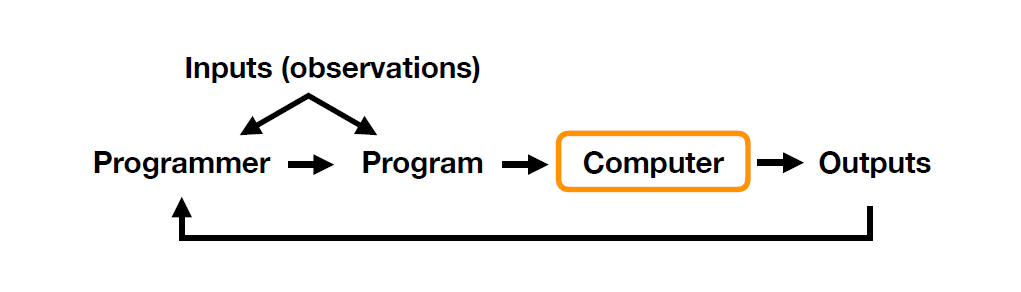
\includegraphics[scale=0.5]{1}
\caption{Classical Programming Paradigm \href{https://sebastianraschka.com/faq/docs/datascience-ml.html}{source}.}
\end{figure}
\end{center}
\end{itemize}
\end{frame}


\begin{frame}{Machine Learning: An Overview}
\begin{itemize}
\item The preceding traditional programming paradigm has several disadvantages:
	\begin{itemize}
	\item what if we don't know waht program should we write for the given data (inputs) ?
	\item what if the inputs change dynamically over the time? should we write another program? 
	\end{itemize}
\item In order to resolve such problems, we should replace the need of developing computer programs "manually"
\item In other words, we would like to automate the process of creating programs by informing the computer, the inputs and outputs that it needs:
\begin{center}
\begin{figure}
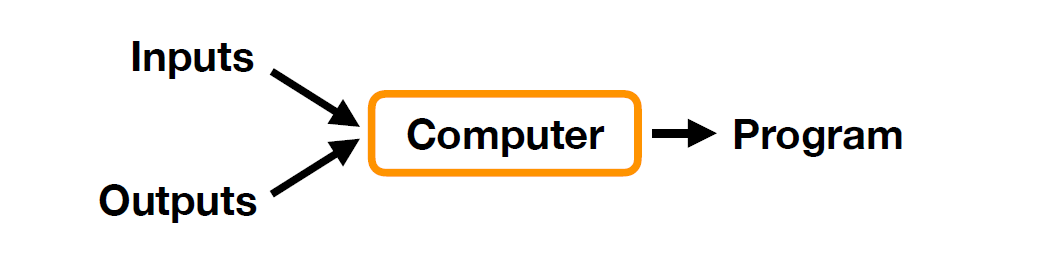
\includegraphics[scale=0.5]{2}
\center \caption{ML Paradigm \href{https://sebastianraschka.com/faq/docs/datascience-ml.html}{source}.}
\end{figure}
\end{center}
\end{itemize}
\end{frame}


%%%%%%%%%%%%%%%%%%%%%%%%%%%%%%%%%%%%%%%%%%%%%%%%%%%%%%%%%%%%%%%%%%%%%%%%%%%%%%%%%%%%%%%%%%%%%%%

%%%%%%%%%%%%%


\begin{frame}{Categories of Machine Learning}
\begin{itemize}
\item The three broad categories of ML are summerized in:
\begin{itemize}
\item \textbf{Supervised Learning}
\item \textbf{Unsupervised Learning}  
\item \textbf{Reinforcement Learning} 
\end{itemize}
\end{itemize}
\begin{figure}
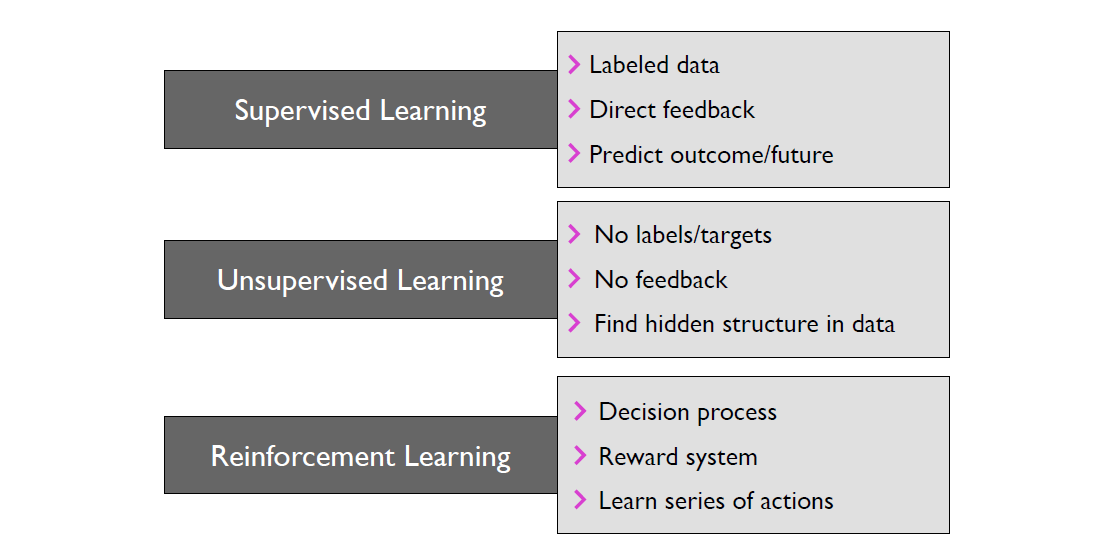
\includegraphics[scale=0.5, right]{3}
\caption{Categories of ML [1].}
\end{figure}
\end{frame}


\begin{frame}{Introduction to Supervised Learning}
\begin{itemize}
\item Supervised learning is the subcategory of machine learning that focuses on learning from labeled training data, our main goal in supervised learning is summerized in one of these categories:
\begin{itemize}
\item \textbf{Classification}: predicting the discrete values such as male/female, etc.
\item \textbf{Regression}: predicting the continuous values such as price, age, etc.
\end{itemize}
\end{itemize}
\begin{columns}
\begin{column}{0.5\textwidth}
\begin{figure}
 \centering
 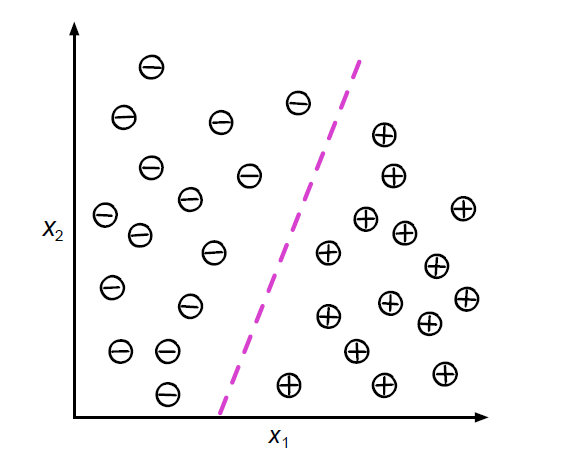
\includegraphics[scale=0.5]{10}  
 \caption{Illustration of Classification Problem [1].}
\end{figure}
\end{column}
\begin{column}{0.5\textwidth}
\begin{figure}
 \centering
 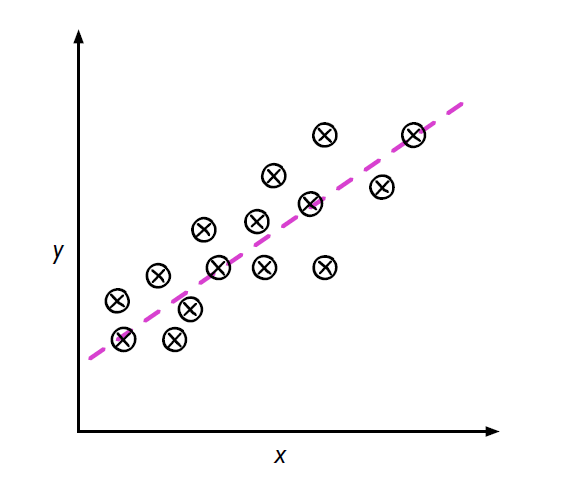
\includegraphics[scale=0.5]{11}  
 \caption{Illustration of Regression Model [1].}
\end{figure}
\end{column}
\end{columns}
\end{frame}

\begin{frame}{Supervised Learning}
\begin{itemize}
\item Given a data set $ \mathcal{D} = \{ \langle \mathbf{x_{\mathnormal 1}} , y_{1} \rangle, \langle \mathbf{x_{\mathnormal 2}} , y_{2} \rangle, \dots, \langle \mathbf{x_{\mathnormal n}} , y_{n} \rangle\} $, there exists an unkown function called $ f $ which:
$$ y = f(\mathbf{x})$$
\item The supervised learning final goal is to \textbf{Approximate} this unkown function. we call our discovery function a \textit{hypothesis} and we define it:
$$  \begin{cases}
       h: \mathbb{R^{\mathnormal m}} \rightarrow \mathbb{R} \\
       h(\mathbf{x}) = y  
  \end{cases} $$
\end{itemize}
\end{frame}

\begin{frame}{Unsupervised Learning}
\begin{itemize}
\item In contrast to supervised learning, unsupervised learning is a branch of machine learning that is concerned with unlabeled data. Common tasks in unsupervised learning are \textbf{Clustering} analysis and \textbf{Dimensionality Reduction}.
\end{itemize}
\begin{columns}
\begin{column}{0.4\textwidth}
\begin{figure}
 \centering
 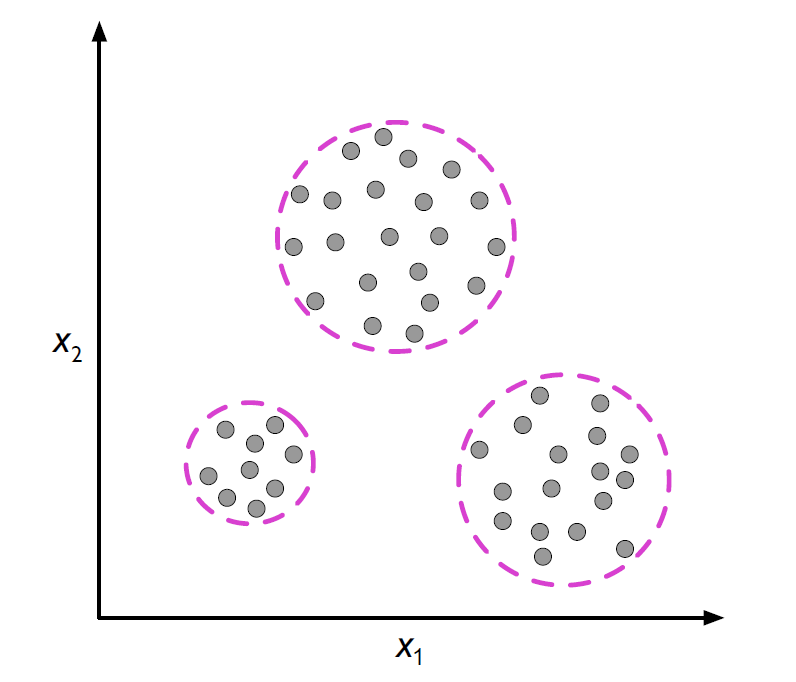
\includegraphics[scale=0.25]{14}  
 \caption{Illustration of Clustering [1].}
\end{figure}
\end{column}
\begin{column}{0.6\textwidth}
\begin{figure}
 \centering
 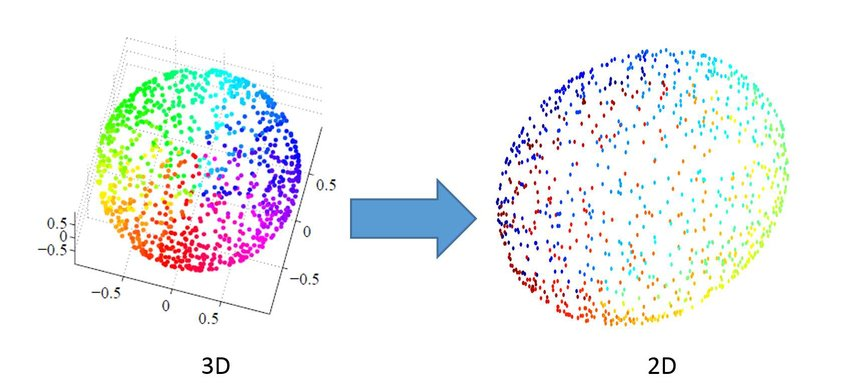
\includegraphics[scale=0.25]{16}  
 \caption{Illustration of Dimensionality Reduction \href{https://www.researchgate.net/figure/Dimensionality-reduction-effect-over-an-artificial-3-dimensional-spherical-shell_fig1_313787026}{source}.}
\end{figure}
\end{column}
\end{columns}
\end{frame}

\begin{frame}{Reinforcement Learning}
\begin{itemize}
\item Reinforcement is the process of learning from rewards while performing a series of actions.
\end{itemize}
\begin{figure}
 \centering
 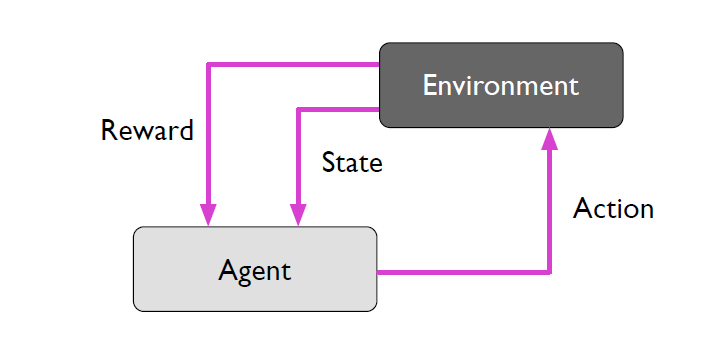
\includegraphics[scale=0.75]{15}  
 \caption{Illustration of Reinforcement Learning [1].}
\end{figure}
\end{frame}

\begin{frame}{Classes of Machine Learning Algorithms}
\begin{itemize}
\item Generalized linear models (e.g., logistic regression)
\item Support vector machines (e.g., linear SVM, RBF-kernel SVM)
\item Artificial neural networks (e.g., multi-layer perceptrons)
\item Tree- or rule-based models (e.g., decision trees)
\item Graphical models (e.g., Bayesian networks)
\item Ensembles (e.g., Random Forest)
\item Instance-based learners (e.g., K-nearest neighbors)
\end{itemize}
\end{frame}

\begin{frame}{Classes of Machine Learning Algorithms}
\begin{figure}
	\begin{subfigure}{0.16\textwidth}
\centering
 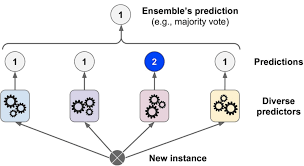
\includegraphics[scale=0.25]{24}  
 \caption{Ensemble Learning \href{https://vitalflux.com/5-common-ensemble-methods-in-machine-learning/}{source}.}
	\end{subfigure}
          \hfill
	\begin{subfigure}{0.16\textwidth}
\centering
 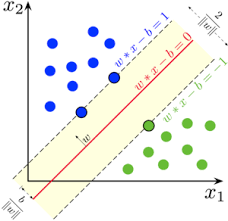
\includegraphics[scale=0.25]{20}  
 \caption{Support Vector Machine \href{https://en.wikipedia.org/wiki/Support-vector_machine}{source}.}
	\end{subfigure}
	\hfill
\begin{subfigure}{0.16\textwidth}
\centering
 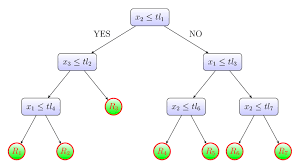
\includegraphics[scale=0.25]{21}  
 \caption{Decision Tree \href{https://www.researchgate.net/figure/Schematic-of-a-Decision-Tree-The-figure-shows-an-example-of-a-decision-tree-with-3_fig1_348456545}{source}.}
	\end{subfigure}
	\hfill
\begin{subfigure}{0.16\textwidth}
\centering
 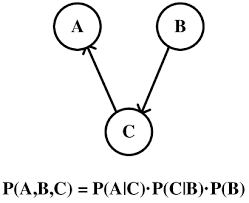
\includegraphics[scale=0.25]{25}  
 \caption{Graphical Models \href{https://www.researchgate.net/figure/Simple-directed-graphical-model-with-three-variables-To-illustrate-how-graphical-models_fig6_262407302}{source}.}
	\end{subfigure}
	\vfill
\begin{subfigure}{0.16\textwidth}
\centering
 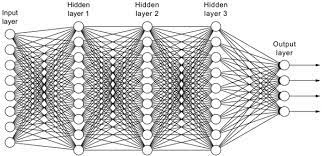
\includegraphics[scale=0.25]{22}  
 \caption{Neural Networks \href{https://www.spiceworks.com/tech/artificial-intelligence/articles/what-is-a-neural-network/}{source}.}
	\end{subfigure}
	\hfill
\begin{subfigure}{0.16\textwidth}
\centering
 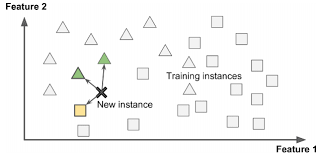
\includegraphics[scale=0.25]{23}  
 \caption{K-Nearest Neighbors \href{https://medium.com/@sanidhyaagrawal08/what-is-instance-based-learning-a9b06079e836}{source}.}
	\end{subfigure}
	\hfill
\begin{subfigure}{0.16\textwidth}
\centering
 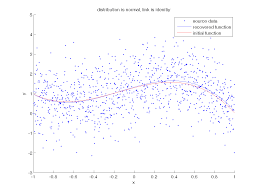
\includegraphics[scale=0.25]{19}  
 \caption{Generalized Linear Models \href{http://strijov.com/sources/demo_GLM.php}{source}.}
	\end{subfigure}
\end{figure}
\end{frame}


\begin{frame}{Algorithm Categorization Schemes}
\begin{itemize}
\item Eager vs Lazy
\item Single-Task vs Multi-Task
\item Generative vs Discriminant
\item Instance-Based vs Model-Based
\item Parametric vs Non-Parametric
\item Batch vs Online
\end{itemize}
\end{frame}

\begin{frame}{5 Steps To Solve A Machine Learning Problem}
\begin{itemize}
\item 1. Define the problem to be solved.
\item 2. Collect (labeled) data.
\item 3. Choose an algorithm class.
\item 4. Choose an optimization metric for learning the model.
\item 5. Choose a metric for evaluating the model.
\end{itemize}
\begin{figure}
 \centering
 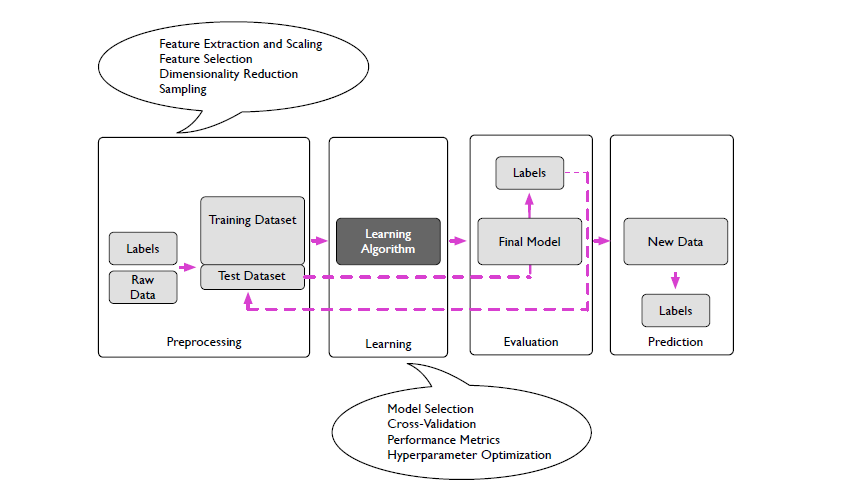
\includegraphics[scale=0.6]{13}  
 \caption{Learning Process [1].}
\end{figure}
\end{frame}

\begin{frame}{Objective Functions}
\begin{itemize}
\item Maximize the posterior probabilities (e.g., naive Bayes)
\item Maximize a fitness function (genetic programming)
\item Maximize the total reward/value function (reinforcement learning)
\item Maximize information gain/minimize child node impurities (CART decision tree classification)
\item Minimize a mean squared error cost (or loss) function (CART, decision tree regression, linear regression, adaptive linear neurons, ...)
\item Maximize log-likelihood or minimize cross-entropy loss (or cost) function
\item Minimize hinge loss (support vector machine)
\end{itemize}
\end{frame}


\begin{frame}{Optimization Methods}
\begin{columns}
\begin{column}{0.5\textwidth}
\begin{itemize}
\item Combinatorial search, greedy search (e.g., decision trees over, not within nodes);
\item Unconstrained convex optimization (e.g., logistic regression);
\item Constrained convex optimization (e.g., SVM);
\item Nonconvex optimization, here: using backpropagation, chain rule, reverse autodi. (e.g., neural networks).
\item Constrained nonconvex optimization (semi-adversarial networks, not covered in this course)
\end{itemize}
\end{column}
\begin{column}{0.5\textwidth}
\begin{figure}
\centering
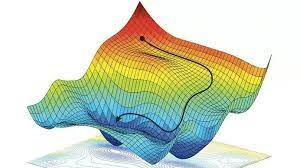
\includegraphics[scale=0.35]{17}  
 \caption{Gradient Descent \href{https://mpalaourg.me/project/optimization-algorithms}{source}.}
\end{figure}
\begin{figure}
\centering
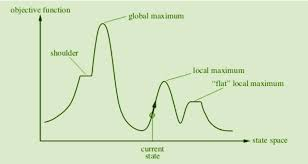
\includegraphics[scale=0.35]{26}  
 \caption{Hill Climbing \href{https://www.geeksforgeeks.org/introduction-hill-climbing-artificial-intelligence/}{source}.}
\end{figure}
\end{column}
\end{columns}
\end{frame}

\begin{frame}{Evaluation}
\begin{itemize}
\item There are several different evaluation metric to assess the performance of a
model, some of them are:
	\begin{itemize}
		\item Accuracy (1-Error)
                   \item ROC AUC
                   \item Precision
                   \item Recall
                    \item (Cross) Entropy
                   \item Likelihood
                    \item Mean Squared Error (MSE)
		\item Mean Absolute Error (MAE)
                    \item L-norms
                   \item ...
	\end{itemize}
\end{itemize}
\end{frame}


%%%%%%%%%%%%%%%%%%%%%%%%%%%%%%
\begin{frame}{Glossary}
\begin{itemize}
\item \textbf{Training example}: A row in the table representing the dataset.
\item \textbf{Training}: Model fitting, for parametric models similar to parameter estimation.
\item \textbf{Feature, $x$}: A column in the table representing the dataset.
\item \textbf{Predicted output, $\hat{y}$}: Use this to distinguish from targets; here, means output from the model.
\item \textbf{Loss function}: Often used synonymously with cost function.
\item \textbf{Hypothesis:}: A hypothesis is a certain function that we believe (or hope) is similar to the true function.
\item \textbf{Classifier}: A classifier is a special case of a hypothesis (nowadays, often learned by a machine learning algorithm). A classifier is a hypothesis or discrete-valued function that is used to assign (categorical) class labels to particular data points. 
\item \textbf{Hyperparameters}: Hyperparameters are the \textit{tuning parameters} of a machine learning algorithm.
\item \textbf{Model}: In the machine learning field, the terms \textit{hypothesis} and \textit{model} are often used interchangeably. In other sciences, they can have different meanings: A hypothesis could be the "educated guess" by the scientist, and the model would be the manifestation of this guess to test this hypothesis.
\item \textbf{Learning algorithm}: Again, our goal is to find or approximate the target function, and the learning algorithm is a set of instructions that tries to model the target function using our training dataset.
\end{itemize}
\end{frame}


\begin{frame}{References}
\begin{itemize}
\item{} \textbf{[1]}. \textit{Raschka, Sebastian, and Vahid Mirjalili. Python Machine Learning: Machine Learning and Deep Learning With Python, Scikit-learn, and TensorFlow 2, 3rd Edition. 3rd ed., Packt Publishing, 2019.}
\end{itemize}
\end{frame}




\frametitle{Final Notes}
\centering
\vspace{50 pt}
\textbf{Thank You!}
\vspace{50pt}

\textbf{Any Question?}
%%%%%%%%%%%%%%%%%%%%%%%%%%%%%%%%%%%%%%%%%%
\end{document}